% Chapter methods

\chapter{Methods} % Main chapter title

\label{Chapter5} % For referencing the chapter elsewhere, use \ref{Chapter5} 

%----------------------------------------------------------------------------------------

% Define some commands to keep the formatting separated from the content 
\newcommand{\keyword}[1]{\textbf{#1}}
\newcommand{\tabhead}[1]{\textbf{#1}}
\newcommand{\code}[1]{\texttt{#1}}
\newcommand{\file}[1]{\texttt{\bfseries#1}}
\newcommand{\option}[1]{\texttt{\itshape#1}}

%~~~~~~~~~~~~~~~~~~~~~~~~~~~~~~~~~~~~~~~~~~~~~~~~~~~~~~~~~~~~~~~~~~~~~~~~~~~~~~~~~~~~~~~






\section{Data and sample collection.} Study material consisted in blood and embryos from the mothers and was collected at the Section Unit of Obstetrics and Gynecology at the University Hospital of Ferrara from 2016 to 2018. The study was approved by the ethical committee of the Emilia-Romagna (CE/FE170475 G.R Reg. E/R (PRUA1GR-2013 00000220 “Silent Intrauterine infections and early pregnancy loss”) and was carried out in compliance with the Helsinki Declaration. All participants provided written informed consents prior to recruitment. All patient data were anonymized right after data and sample collection.\\ 

Data were cleaned and refined (e.g.trimming of white spaces, correction of typing errors, harmonization of values within fields, and similar) using OpenRefine (\url{https://github.com/OpenRefine/OpenRefine}), a standalone open source application for data cleanup and transformation (\href{https://en.wikipedia.org/wiki/OpenRefine}{wiki}).\\

Summary statistics of the data and hypothesis testing were calculated and represented using the packages \textit{ggplot} \cite{ggplot2}, \textit{tidyverse} \cite{wickham2019welcome}, \textit{stats} \cite{statsR} and \textsc{r} \cite{R}. All the code is available on the git repository of the project (\url{https://github.com/ezcn/grep}) 

\section{Screening for chromosomal aneuploidies}

This part was performed by our collaborators at the University of Ferrara and Merigen Reserach s.r.l. In brief DNA was extracted from chorionic villi of the product of conception using standard protocols. A rapid screening of sex and numerical anomalies for chromosomes 13, 15, 16, 18, 21, 22 and X was carried out with the miscarriage DNA samples performing quantitative PCR assays. Samples that resulted euploid for these chromosomes were further analized by Comparative Genomic Hybridization (Agilent SurePrint G3) and low coverage sequencing of randomly amplified genomic regions


\section {Whole-genome sequence analyses}

\subsection{Sequencing}
Sequencing was done through a service provider (Macrogen s.r.l). In particular, libraries for sequencing were prepared using the Illumina TruSeq DNA PCR-free Library (insert size 350bp) and samples were sequenced at 30X mapped (~110Gb) 150bp PE on HiSeqX. Data were released in as fastq files. 

\subsection{Alignment with reference.} Reads in the fastq file were aligned against the reference genome GRChg38.p12 \cite{rosenbloom2015ucsc} using \textsc{bwa} and \textsc{samtools}. \textsc{bwa} (\url{https://github.com/lh3/bwa}) "is a software package for mapping low-divergent sequences against a large reference genome, such as the human genome." Of the three algorithms available in \textsc{bwa} we used \textsc{bwa-mem}  that is generally recommended to analyze 70-100bp Illumina reads.\\

Downstream to \textsc{bwa-mem} I used \textsc{samtools} (\url{https://github.com/samtools/samtools}) to obtain a BAM from a fastq. \textsc{samtools} "is a set of utilities for interacting with and post-processing short DNA sequence read alignments in the SAM (Sequence Alignment/Map), BAM (Binary Alignment/Map) and CRAM formats" (\href{https://en.wikipedia.org/wiki/SAMtools}{wiki}). 

For each sample, the following command line takes in input fastq file (paired-end) and gives as output a raw-bam file that contains the alignment of the reads against the reference genome: 

\begin{verbatim}
~/bin/bwa mem -t 16 -R "@RG\tID:$idsample\tSM:$idsample" \
/mpbastudies3/IMMA/hg38/hg38.p12.fa \ 
/mpbastudies3/181113_Vincenza-Colonna/$namedir/$nameflgz1 \ 
/mpbastudies3/181113_Vincenza-Colonna/$namedir/$nameflgz2 | \ 
/mpba0/mpba-sw/samtools view -b - > \
/mpbastudies3/IMMA/samples/$idsample.raw.bam
\end{verbatim}


\subsection{Refining}
The  process of library preparation prior to sequencing can introduce artifacts such as PCR duplications. Although the type of library used for the sequencing of the GREP samples is PCR-free we checked for PCR duplicates using the function markdup of \textsc{sambamba}. As expected we did non find replicates. 

SAMbamba (\url{https://github.com/biod/sambamba}) \textit{"is a high performance highly parallel robust and fast tool (and library), written in the D programming language, for working with SAM and BAM files"}  (\href{https://github.com/biod/sambamba#introduction}{git}).

The command line takes as input a raw version of the BAM file for each sample and gives as output a BAM file without PCR duplicates:  

\begin{verbatim}
~/bin/sambamba markdup -t 8 -p  \
--tmpdir /scratch --overflow-list-size 500000 \
/mpbastudies3/IMMA/samples/${idflrbam}.raw.sorted.bam \
/mpbastudies3/IMMA/samples/${idflrbam}.bam    
\end{verbatim}


\subsection{Variant calling} 
The variant calling identifies sites of an individual genome that differ from the reference sequence. We used \textsc{freebayes} (\url{https://github.com/ekg/freebayes}) that is "a Bayesian genetic variant detector designed to find small polymorphisms, specifically SNPs (single-nucleotide polymorphisms), indels (insertions and deletions), MNPs (multi-nucleotide polymorphisms), and complex events (composite insertion and substitution events) smaller than the length of a short-read sequencing alignment." (\href{https://github.com/ekg/freebayes}{git}).
\textsc{freebayes} requires the reference genome in fasta format and the BAM file for each sample. To speedup the process I did independent analysis for each chromosome for each individual. The command line that I used is: 

\begin{verbatim}
~/bin/freebayes -f /mpbastudies3/IMMA/hg38/hg38.p12.fa \ 
-r ${chr} --gvcf -g 2000  /mpbastudies3/IMMA/samples/${idsample}.bam 
\end{verbatim}

\subsection {Compress and indexing.} 
vcf files generated by \textsc{freebayes} are compressed and indexed. Compression optimizes files storage and transfer. Indexing allows fast access to large files. 

Compression was done using Bgzip (\url{https://www.htslib.org/doc/bgzip.html#DESCRIPTION}) that "compresses files into a series of small (less than 64K) 'BGZF' blocks. This allows indexes to be built against the compressed file and used to retrieve portions of the data without having to decompress the entire file" (\href{https://www.htslib.org/doc/bgzip.html#DESCRIPTION}{wiki}).
The command line takes in input the output (VCF) from variant calling and outputs the compressed file: 

\begin{verbatim}
~/bin/bgzip /mpbastudies3/IMMA/samples/vcf/${idsample}.vcf > \
/mpbastudies3/IMMA/samples/vcf/${idsample}.vcf.gz
\end{verbatim}

Indexing was done using Tabix (\url{https://www.htslib.org/doc/tabix.html}) that "indexes a TAB-delimited genome position file in.tab.bgz and creates an index file". The command line takes in input the compressed file from BGZIP and produces an indexed file: 

\begin{verbatim}
~/bin/tabix -p vcf /mpbastudies3/IMMA/samples/vcf/${id}.${chr}.vcf.gz 
\end{verbatim}


\subsection{Variant Effect Predictor.}  
VEP (\url{https://grch37.ensembl.org/info/docs/tools/vep/index.html}) determines the effect of genetic variants (SNPs, insertions, deletions, CNVs or structural variants) on genes, transcripts, and protein sequence, as well as regulatory regions. \textsc{vep} takes as input the coordinates of the variants and the nucleotide changes to find out the:
\begin{itemize}
    \item Alleles, Genes and Transcripts affected by the variants
    \item Location of the variants (e.g. upstream of a transcript, in coding sequence, in non-coding RNA, in regulatory regions)
    \item Consequence of the variation on the protein sequence (e.g. stop gained, missense, stop lost, frameshift)
    \item Matches with known variants, and associated  allele frequencies from databases of human sequences
    \item Several scores associated to changes to the protein sequence
\end{itemize}

\textsc{vep} takes in input a refined vcf file and gives as output an annotated vcf or a json file with information for all the parameters written in the command-line. I used the \textsc{vep} version 96.3 with the following command-line: 

\begin{verbatim}
singularity run -B /mpbastudies3/IMMA/samples/:/data \
/mpba0/mpba-sw/biocontainers/vep-96.3.img \
--af_1kg --af_gnomad --appris --biotype \
--buffer_size 5000 --check_existing --distance 5000 \
--fork 4 --polyphen b --pubmed --regulatory --sift b \
--species homo_sapiens --symbol --tsl --cache \
--dir_cache /mpba0/vcolonna/vepcache/ --offline \
--vcf --variant_class -i /data/vcfconcat/${id}.fullVcf \
-o /data/vepVCF/${id}.fullvep
\end{verbatim}

\subsection{Filtering and ranking using custom Python scripting}
    
\begin{figure}[H]
\centering
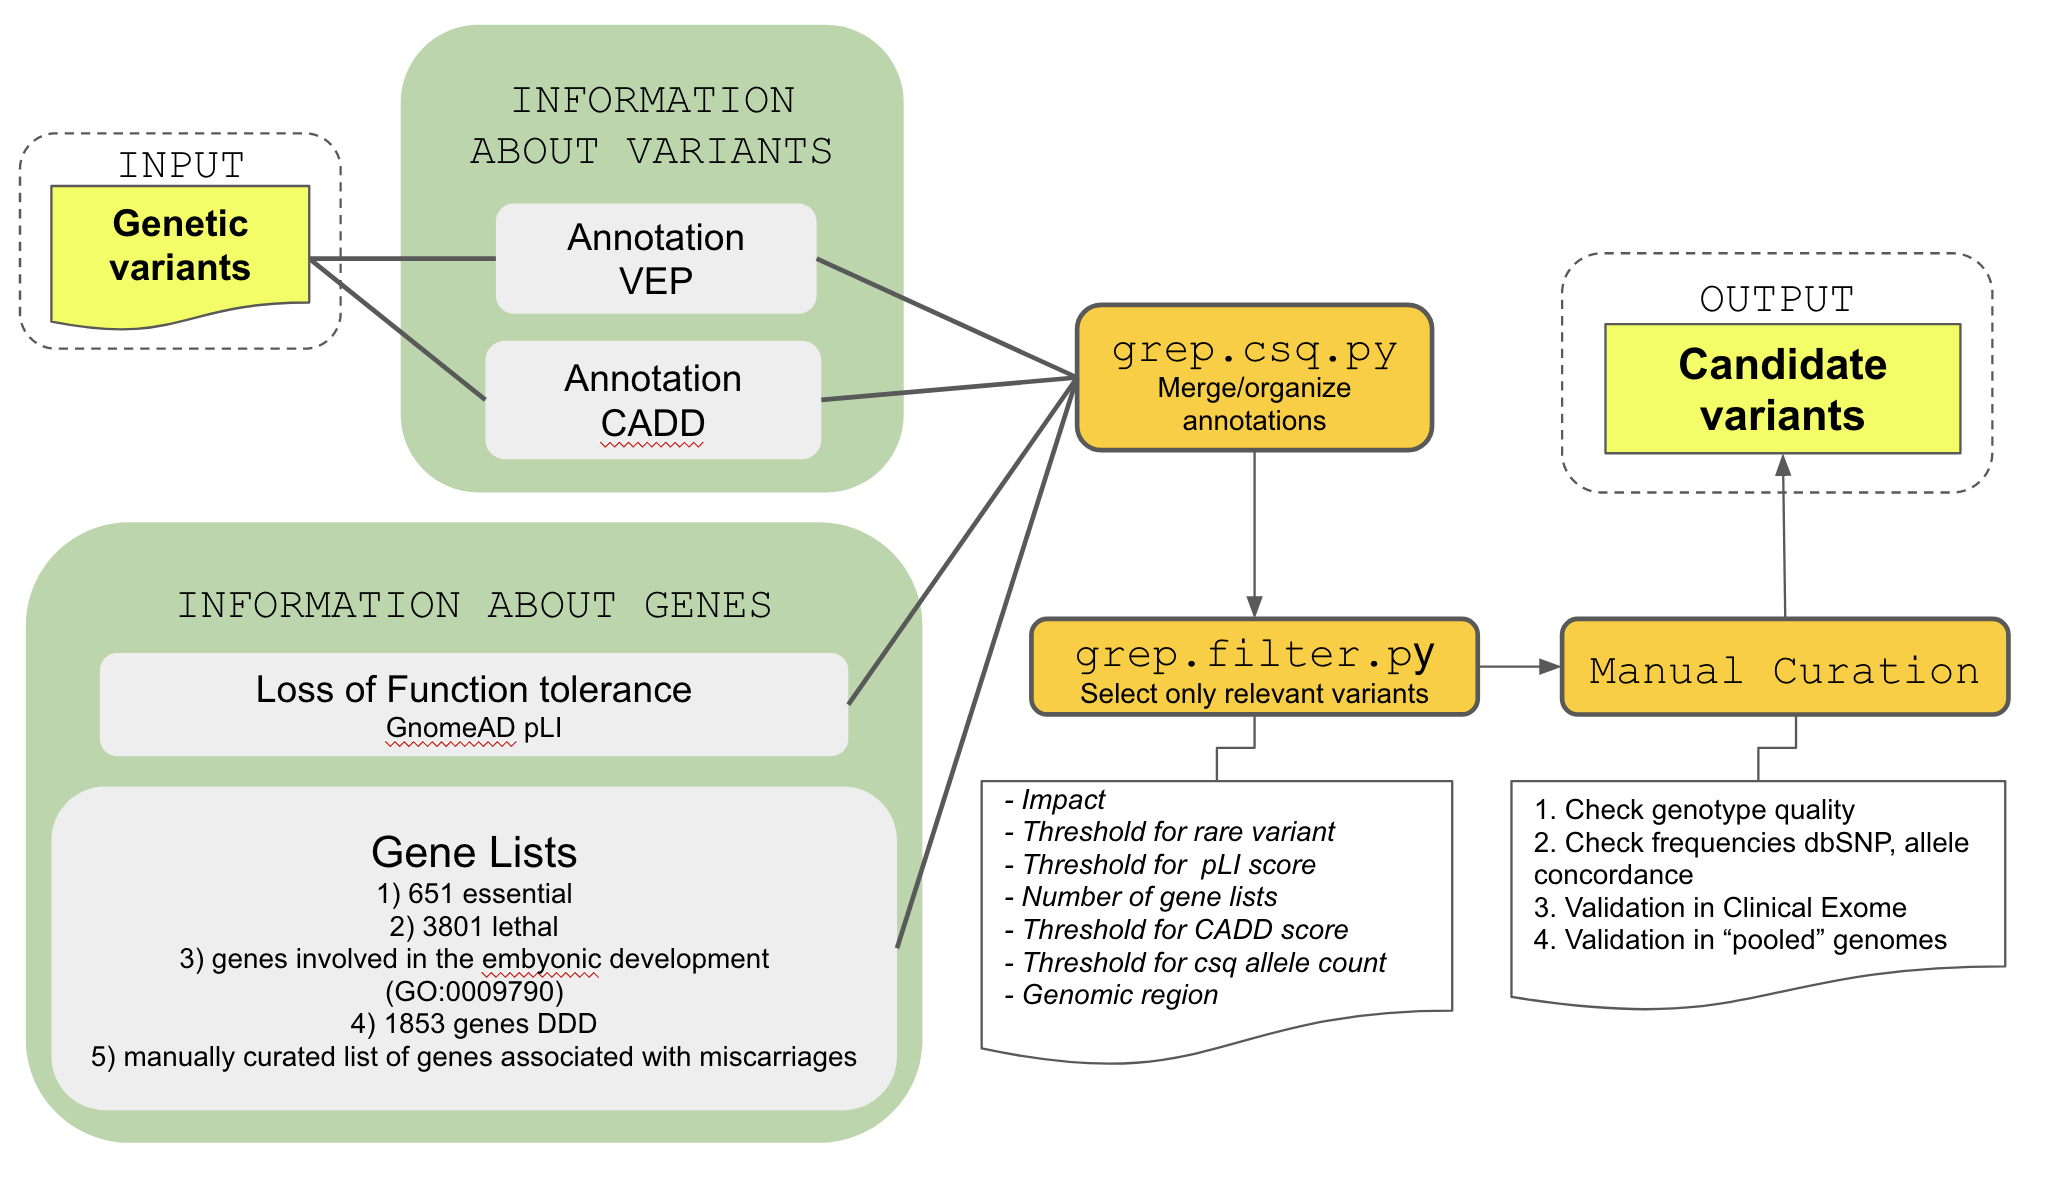
\includegraphics[width=0.95\textwidth]{fig/pipelineComplete.png}
\decoRule
\caption{\textbf{Our pipeline (\url{https://github.com/ezcn/grep})} is written in Python and in consists of two script. The first one (\textsc{grep.csq.py}) takes as input a file with the genomic location of the genetic variants and annotates it with the information from several databases on genetic variants and genes. The second (\textsc{grep.filter.py}) selects only relevant variants according to the filters specified by the user. The results of \textsc{grep.filter.py} are manually curated to obtain the candidate variants.} 
\label{fig:pipelineComplete}
\end{figure}


\subsection{Tools for High Performance Computing}

\subsubsection{Containers}
In the last few years the attention of programming world was moving to containers that are standard units of software that consist to package all the \gls{code} and \gls{dependencies} and allow to runs the packaged-software quickly and reliably from one computing environment to another. I have used two type of this containers, \textsc{singularity} \cite{kurtzer2017singularity} and \textsc{docker} \cite{merkel2014docker}. \textsc{singularity} have more flexibility than \textsc{docker} but defect stability and don't already have a big community of users and developers.

\subsubsection{Workload management systems}
All the analysis was made on remote HPC machine that use two software for parallelization of computationally intensive tasks \textsc{sgl} \cite{} and \textsc{htcondor}\cite{condor-practice}. \textsc{htcondor} was preferred to \textsc{sgl} for intensive and high computational tasks. \textsc{sgl} was used for simple and single core tasks.

\subsubsection{Programming languages}
I learned and used bash \cite{gnu2007free}, awk \cite{aho1979awk}, Python \cite{python3} 

